
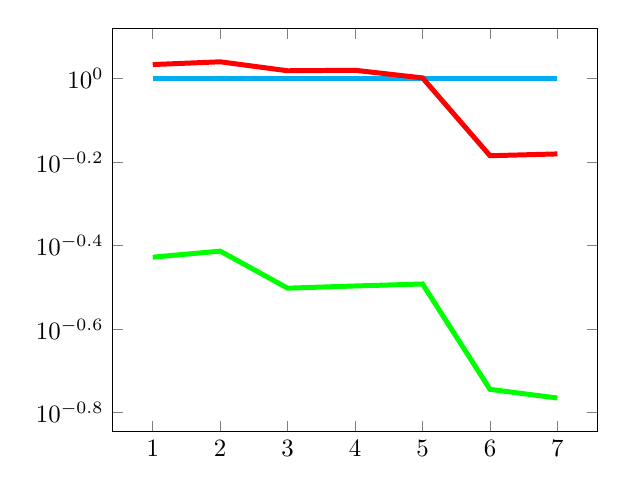
\begin{tikzpicture}[scale=0.9]
\begin{semilogyaxis}
\addplot[color=cyan,line width=2pt] coordinates {(1,1.0)(2,1.0)(3,1.0)(4,1.0)(5,1.0)(6,1.0)(7,1.0)};
\addplot[color=red,line width=2pt] coordinates {(1,1.0794172305264202)(2,1.0960491971389397)(3,1.0431971998882215)(4,1.0459819355719462)(5,1.0028021188535186)(6,0.6531686519848551)(7,0.6597339093819087)};
\addplot[color=green,line width=2pt] coordinates {(1,0.37346383954653894)(2,0.38616179420290614)(3,0.31481250115792014)(4,0.3186641663934093)(5,0.32215220073737655)(6,0.18023779125078165)(7,0.1718313423550623)};

\end{semilogyaxis}
\end{tikzpicture}
